\documentclass{article}
\usepackage{graphicx} % Required for inserting images
\usepackage{amsmath}

\title{GNSS Signal Modeling}
\author{Brian Breitsch}
\date{December 2025}

\begin{document}

\maketitle

\section{Introduction}

This document derives the signal model for a transmitted/received GNSS signal.  The model may be useful for processing received signals as well as for simulating or analyzing signal parameters under different scenarios.

\section{Signal Model Derivation}

\subsection{Time Scale Definitions}

In order to provide a comprehensive signal model, we must begin with a description of the receiver and transmitter oscillators and clocks:
%
\begin{align}
t_\text{tx}(t) = t + \Delta t_\text{tx}(t)  \\
t_\text{rx}(t) = t + \Delta t_\text{rx}(t)
\end{align}
%
Here, the transmitter and receiver clock errors are denoted $\Delta t_\text{tx}(t)$ and $\Delta t_\text{rx}(t)$, and are defined relative to a reference timescale $t$ (e.g. GPS system time).  Later, it will be helpful to have also defined the clock drifts $d_\text{tx}$ and $d_\text{rx}$ (again, measured relative to the reference time scale):
%
\begin{align}
\frac{\partial t_\text{tx}}{\partial t}(t) &= 1 + \frac{\partial \Delta t_\text{tx}}{\partial t}(t) = 1 + d_\text{tx}(t)  \\
\frac{\partial t_\text{rx}}{\partial t}(t) &= 1 + \frac{\partial \Delta t_\text{rx}}{\partial t}(t) = 1 + d_\text{rx}(t)
\end{align}
%

\subsection{Transmitted Signal}

Transmitted GNSS signals can be modeled as quadrature modulated carriers that are synchronized to the transmitter clock:
%
\begin{align}
s_\text{tx}(t) = A_\text{tx} \cdot \left[ C_I(t_\text{tx}(t)) \cdot \text{cos}\left( \omega_c \cdot t_\text{tx}(t) \right) +C_Q(t_\text{tx}(t))\cdot\sin(\omega_c \cdot t_\text{tx}(t)) \right]
\end{align}
%
Here
%
\begin{itemize}
    \item $A_\text{tx}$ is the transmitted signal amplitude
    \item $C_{I/Q}(\cdot)$ are in-phase and quadrature-phase modulation code sequences
    \item $\omega_c$ is the carrier angular frequency (e.g. $2\pi \cdot 1575.42$ MHz for GPS L1)
\end{itemize}




\subsection{Idealized Propagation and Reception}

This signal propagates through a noisy channel, characterized by a time-varying impulse response, which may include the effects of range delay, atmospheric delays and distortions, surface reflections and multipath, and transmitter and receiver hardware distortions.  In the simplest, ideal case, this response is modeled as an attenuated delay $h(t,\tau) = \alpha(t) \delta(\tau - \tau_\text{prop}(t))$, where:
\begin{itemize}
    \item $\alpha(t)$ characterizes the signal attenuation
    \item $\delta(\cdot)$ is the delta distribution
    \item $\tau_\text{prop}(\cdot)$ denotes the channel propagation delay, or signal ``travel time,'' which accounts for range delay, transmitter and receiver biases that are distinct from the transmitter/receiver clock models, and atmospheric delays
\end{itemize}
%
Note that more complicated channel impulse responses, e.g. due to multipath or scattering, can often be expressed as a sum of this simple response over different delays with varying complex amplitudes.  Dispersive effects (e.g. ionosphere effects) are a different story, and will be dealt with later.

In the simple case, after the signal is received (but before mixdown) we have:
%
\begin{align*}
s_\text{rx}'(t) &= \left(s_\text{tx} * h\right)(t) + \epsilon_\text{rx}'(t)  \\
&= \alpha(t) \cdot A_\text{tx} \cdot \left[ C_I(t_\text{tx}(t-\tau_\text{prop}(t))) \cdot \text{cos}\left( \omega_c \cdot t_\text{tx}(t-\tau_\text{prop}(t)) \right) \right. \\ & \hspace{5mm} \left. + \ C_Q(t_\text{tx}(t-\tau_\text{prop}(t)))\cdot\sin(\omega_c \cdot t_\text{tx}(t-\tau_\text{prop}(t))) \right] + \epsilon_\text{rx}'(t)
\end{align*}
%
The receiver radio front-end typically performs one or more analog or digital mixdown stages, whose net effect can be modeled as an additional attenuation (optimally $\frac{1}{2}$) and multiplication with a locally-generated complex sinusoid of frequency $\omega_c$.  After mixdown our ideal received \textit{baseband} signal model can be expressed:
%
\begin{align}
    s_\text{rx}(t) &= \frac{1}{2} \cdot s_\text{rx}'(t) \cdot \exp(-j\cdot \omega_c \cdot t_\text{rx}(t))  \nonumber \\
    &= A_\text{rx}(t) \cdot \left[ C_I (\eta(t)) + j \cdot C_Q(\eta(t)) \right] \cdot \text{exp}\left( j \phi(t) \right)  + \epsilon_\text{rx}(t)
\end{align}
% &= A_\text{rx}(t) \cdot C(\eta_\text{rx}(t)) \cdot \text{exp}\left( i \phi_\text{rx}(t) \right)  + \epsilon_\text{rx}(t)
% &= A_\text{rx}(t) \cdot C(\eta(t)) \cdot \text{exp}\left( i \phi(t) \right)  + \epsilon_\text{rx}(t)
% \end{align*}
%
where here we introduce the following terms:
\begin{itemize}
    \item $A_\text{rx}(t)$ is the baseband received signal amplitude
    \item $\eta(t)$ is the received signal code phase (typically in units of chips, seconds, or milliseconds)
    \item $\phi(t)$ is the baseband received signal carrier phase (in radians)
    \item $\epsilon_\text{rx}(t)$ is an approximately white noise term, often modeled as drawn from a complex Gaussian, which accounts for both the receiver noise temperature and the antenna sky noise.
\end{itemize}



\subsection{Signal Parameter and Measurement Definitions}

Typical receiver signal processing aims to measure the carrier phase, code phase, and amplitude as expressed in this baseband signal model.  In particular, when converted to a delay in units of meters, the measured code phase is often referred to as the ``pseudorange'' and the measured carrier phase ($\Phi(t)=-\frac{c}{\omega_c}\cdot\phi(t)$) is called the ``accumulated Doppler range,'' or ADR.

An \textit{ideal} pseudorange $\rho$ is defined as the speed of light $c$ multiplied by the difference between the receiver's time of reception, $t_\text{rx}(t)$, and the transmitter's time of transmission, $t_\text{tx}(t-\tau_\text{prop}(t))$:
%
\begin{align}
\rho(t) &= c \cdot \left(t_\text{rx}(t) - t_\text{tx}(t - \tau_\text{prop}(t)) \right)  \\
&= c \cdot \left(\tau_\text{prop}(t) + \Delta t_\text{rx}(t) - \Delta t_\text{tx}(t - \tau_\text{prop}(t)) \right)
\end{align}
%
Note that, for the ideal channel response, pseudorange can be measured directly from the \textit{measured signal delay} $\tau_\rho$, where $\rho(t)=c\cdot \tau_\rho(t)$ and:
%
\begin{align}
    \eta(t) = t_\text{tx}(t-\tau_\text{prop}(t)) = t_\text{rx}(t) - \tau_\rho(t)
    \label{eqn:ideal-code-phase}
\end{align}
%
In the non-dispersive case, the carrier phase shares the dynamics that are present in $\tau_\rho(t)$:
%
\begin{align}
\phi(t) &= \omega_c\cdot \left[ t_\text{tx}(t-\tau_\text{prop}(t)) - t_\text{rx}(t) \right] + k_c \cdot b_\phi(t)  \nonumber  \\
&= -\omega_c \cdot \tau_\rho(t) + k_c \cdot b_\phi(t)  \\
&= -\omega_c \cdot \tau_\phi(t) \hspace{5mm} \text{where} \hspace{5mm} \tau_\phi(t) = \tau_\rho(t) + \frac{1}{c}\cdot b(t)
\label{eqn:ideal-carrier-phase}
\end{align}
%
Here $b_\phi$ denotes an integer-wavelength ambiguity bias and $k_c=2\pi / \lambda=\omega_c/c$ is the spatial carrier wavenumber.  The term $b_\phi$ is added to emphasize the fact that carrier phase is ambiguous over integer cycles.  We call $\tau_\phi$ the \textit{measured phase delay}.

\subsection{Phase Rate Modeling}
% TODO: move section to signal replica generation
For both code and carrier phase, it is helpful to notate their instantaneous rates of change (i.e. the ``code rate'' and ``carrier rate'').  For rate quantities  measured relative to the reference time scale, we use the overhead dot notation:
%
\begin{align}
    \frac{\partial \tau_\rho}{\partial t}(t) &= \dot{\tau}_\rho(t)  \\
    \frac{\partial \eta}{\partial t}(t) &= \dot{\eta}(t) = 1 + d_\text{rx}(t) - \dot{\tau}_\rho(t)  \\
    \frac{\partial \phi}{\partial t}(t) &= \dot{\phi}(t) = -\omega_c \cdot \dot{\tau}_\rho(t) 
\end{align}
%
When these rates are instead measured relative to the receiver time scale, they obtain a factor of $1/(1+d_\text{rx}(t))$.  For example, the carrier phase rate becomes:
%
% \begin{align}
%     \frac{\partial \eta}{\partial t_\text{rx}}(t) &= \frac{\partial \eta(t)}{\partial t} \frac{\partial t}{\partial t_\text{rx}} = \frac{\dot{\eta}(t)}{1 + d_\text{rx}(t)} = 1 - \frac{\dot{\tau}_d(t)}{1 + d_\text{rx}(t)} \\
% \end{align}
% %
% and
%
\begin{align}
    \frac{\partial \phi}{\partial t_\text{rx}}(t) &= \frac{\partial \phi(t)}{\partial t} \frac{\partial t}{\partial t_\text{rx}} = \frac{\dot{\phi}(t)}{1 + d_\text{rx}(t)} = \omega(t)
\end{align}
%
Here, we use the symbol $\omega(t)$ to specifically refer to the carrier phase rate at time $t$ relative to the receiver (rather than the system) time scale.  This quantity (the \textit{measured} carrier rate) is often referred to as the \textit{angular Doppler frequency}.  With this notation, we then have:
%
\begin{align}
    \frac{\partial \tau_\rho}{\partial t_\text{rx}}(t) &= -\frac{\omega(t)}{\omega_c}  \\
    \frac{\partial \eta}{\partial t_\text{rx}}(t) &= 1 + \frac{\omega(t)}{\omega_c}  \label{eqn:angular-dopp-to-code-rate}
\end{align}
%



\subsection{Receiver Time Coordinates and Sampling}

Thus far, we have described these parameters as functions of the reference or system time $t$.  However, when it comes to the receiver's signal processing and measurements, we must model and timestamp these quantities relative to receiver time epochs.  In typical digital signal processing receivers, the time is defined at each sample according to the nominal sampling rate.  If the epochs of received samples are $\{t_n\}$, the receiver will report them as times $\{ t_\text{rx}(t_n)\}$, which can be expressed as:
%
\begin{align}
t_\text{rx}(t_n) &= t_\text{rx}(t_0) + n \cdot \Delta t_\text{samp}  \\
& \Downarrow \notag \\
t_n &= t_\text{rx}(t_0) + n\cdot\Delta t_\text{samp} - \Delta t_\text{rx}(t_n) 
\end{align}
%
where $t_0$ is some epoch at which the receiver clock value is set.

Let us denote time-varying terms evaluated at time $t_n$ using the notation $(\cdot)[n]$.  Then for the received signal model, we have:
%
\begin{align}
    s_\text{rx}[n] = A_\text{rx}[n] \cdot C(\eta[n]) \cdot \exp(j\cdot \phi[n]) + \epsilon_\text{rx}[n]
    \label{eqn:received-sampled-signal-model}
\end{align}


\section{Signal Processing}

\subsection{Replica Model}

% \begin{align}
%     s_\text{rep}[n]=C(\bar{\eta}[n]) \cdot \exp(j \cdot \bar{\phi}[n])
% \end{align}

% \begin{align}
%     \bar{\eta}[n] = \eta[0] + n \cdot 
% \end{align}

The core operation of GNSS receiver signal processing is to correlate a replica signal with the received signal.  We express this replica as:
% \begin{align}
%     s_\text{rep}(t) = C(\bar{\eta}(t)) \cdot \exp(j\cdot \bar{\phi}(t))
% \end{align}
\begin{align}
    s_\text{rep}[n] = C(\bar{\eta}[n]) \cdot \exp(j\cdot \bar{\phi}[n])
\end{align}
%
where $\bar{\eta}$ and $\bar{\phi}$ denote the modeled (replica) code and carrier phase.  Often these quantities are modeled as linearly varying with respect to the receiver time scale over a particular segment of time (e.g. the correlation interval).  Additionally, the replica code and carrier are typically constrained to have the same rate dynamics (i.e. they follow our ideal, non-dispersive received signal model; in tracking loops this constraint is known as ``carrier aiding''), so we can express the code rate using our angular Doppler as in Equation \ref{eqn:angular-dopp-to-code-rate}.  For a set of epochs $\{t_{n+m}\}$ near some reference epoch $t_n$, our replica code and carrier phase models are:
%
\begin{align}
    % \bar{\eta}[n+m] &= \bar{\eta}[n] + \dot{\bar{\eta}}_d[n] \cdot (t_\text{rx}[m+n] - t_\text{rx}[n])  \\
    % &= \bar{\eta}[n] + \dot{\bar{\eta}}_d[n] \cdot m \cdot \Delta t_\text{samp}  \\
    % &\approx \bar{\eta}(t_0) + \dot{\bar{\eta}}(t_0) \cdot (t_n - t_0)  \\
    \bar{\eta}[n+m]  &= \bar{\eta}[n] + \left(1 + \frac{\bar{\omega}(t)}{\omega_c} \right) \cdot m \cdot \Delta t_\text{samp}  \\
    \bar{\phi}[n+m] &= \bar{\phi}[n] + \bar{\omega}[n] \cdot m \cdot \Delta t_\text{samp}
\end{align}
%
Note, here, that code phase has implicitly been described in units of seconds.

\subsection{Correlation Model}

For a correlation interval of duration $T_I$ corresponding to $M$ samples at times $\{t_{n+m}\}_{m=0}^{M-1}$, the measured correlation output is given by:
%
\begin{align*}
z(t_n) &= \left( s_\text{rx} \star s_\text{rep}\right)_{t_n}^{t_{n+M}}  \\
 &= \sum_{m=0}^{M-1} s_\text{rx}[n+m] \cdot \text{conj}\left(s_\text{rep}[n+m]\right)
\end{align*}
%
We can derive an analytical expression for the correlation result if we make some approximations to our received and replica signal models over the correlation interval.  Specifically, if we assume:
%
\begin{enumerate}
    \item The received signal amplitude is approximately constant ($A_\text{rx}(t_{n+m}) \approx A_\text{rx}(t_n)$)
    \item The received signal code phase nearly matches the replica code phase ($\eta(t)\approx \bar{\eta}(t)$)
\end{enumerate}
%
and/or
%
\begin{enumerate}
    \setcounter{enumi}{2}
    \item The received signal carrier phase rate (Doppler) nearly matches the replica carrier rate ($\bar{\omega}(t)\approx\dot{\phi}(t)$)
\end{enumerate}
%
then we can derive the following expression:
%
\begin{align}
    Z(t_n) \approx A_\text{rx}[n] \cdot M \cdot R(\Delta\eta[n])\cdot \text{sinc} \left( \frac{T_I}{2}\cdot\Delta \omega[n] \right) \cdot \exp\left[ j \left(\Delta \theta[n] \right) \right] + \epsilon[n] \label{eqn:correlation}
\end{align}
% When C(eta) * C(bar{eta}) \approx 1
% then sum_M [ A * exp(j*dphi) ]
%      = A * exp(j*dphi0) * sum_{m=0}^{M-1} [ exp(j * domega * m * Dt) ]
% and using geometric series, we have:
%      = A * exp(j*dphi0) * (1 - exp(j * domega * M * Dt) / (1 - exp(j * domega * Dt))
%      = A * exp(j*dphi0)
%          * exp(j * domega * M / 2 * Dt) / exp(j * domega / 2 * Dt)
%          * sin(domega * M / 2 * Dt) / sin(domega / 2 * Dt)
%      = A * exp(j*dphi0 + j*domega * (M-1) / 2 * Dt)
%          * M * sinc(domega * M / 2 * Dt)
%
where
%
\begin{itemize}
    \item $\Delta\eta[n]$ is the received-replica code phase error (at time $t_n$)
    \item $\Delta\theta[n] = \Delta \phi[n] + \frac{T_I}{2}\cdot \Delta\omega[n] = \angle E[Z(t_n)] $ is the average phase error over the correlation interval
    \item $\Delta\phi[n]$ is the received-replica carrier phase error (at time $t_n$)
    \item $\Delta\omega[n]$ is the received-replica Doppler angular frequency error
    \item $R(\cdot)$ is, nominally, the autocorrelation function of modulation code $C(\cdot)$
    \item $\epsilon[n]$ is a new correlation noise term, which very loosely can be modeled as a sum of the $M$ Gaussian RVs $\{\epsilon_\text{rx}[n+m]\}_{m=0}^{M-1}$
\end{itemize}

Our expression for the correlation value in Equation \ref{eqn:correlation} is also known as the ``cross ambiguity function.''  Note how if either $\Delta\eta \gg \frac{T_\text{chip}}{2}$ or $\Delta\omega \gg \frac{2}{T_I}$ then our signal correlation energy goes to zero and $Z$ becomes dominated by noise.


\section{Dispersion}

A dispersive channel is one where the wave propagation speed depends on the frequency.  In this case, the channel impulse response is no longer a simple attenuated delay, and our received signal model is no longer accurate.  Some channels can lead to distortion in the received signal waveform.  For narrowband signals (such as GPS L1CA and L2C), the waveform distortion is often negligible, particularly for the ionosphere.  However, dispersive media will still introduce group delay and phase effects, which must be modeled slightly differently than the idealized signal model presented thus far.

To illustrate dispersive effects, let us consider the ionospheric propagation channel.  In a first-order approximation, the phase refractive index in the ionosphere at a position $\mathbf{r}$ for a wave with frequency $f$ is:
%
\begin{align}
    n(t,f,\mathbf{r}) \approx 1 - \frac{40.3}{f^2} \cdot N_e(t,r)
\end{align}
%
where $N_e(t,\mathbf{r})$ denotes the temporally and spatially varying ionospheric plasma electron density.  As the signal travels through the ionosphere, this leads to a net phase impact of the ionospheric channel modeled by:
%
\begin{align}
    \frac{c}{\omega_c} \cdot \phi_\text{iono}(t,f) = \int_{\mathbf{r}_\text{tx}}^{\mathbf{r}_\text{rx}} \left( n(t,f,\mathbf{r}) - 1 \right) \cdot d\mathbf{r} = - \frac{40.3}{f^2} \cdot \text{TEC}(t)
\end{align}
%
where $\text{TEC}(t)$ is the path-integrated electron density, or  total electron content.  Note that subtracting 1 from the refractive index in the integrand makes this expression represent the ionospheric impact on the signal propagation, excluding the straight-line prropagation range delay.  This lets us express the effective frequency response of the ionospheric channel as:
%
\begin{align}
    H(t,f) = \exp\left(j \cdot \phi_\text{iono}(t,f)\right) =  \exp \left( -j \frac{2\pi}{c} \cdot \frac{40.3}{f} \cdot \text{TEC}(t) \right)
\end{align}
%
Figure \ref{fig:iono-freq-response} illustrates this transfer function, and Figure \ref{fig:iono-impulse-response} shows the corresponding impulse responses for different values of TEC.  As is typical of dispersive channel impacts on narrowband signals, the impulse response can be essentially modeled as a separate group delay and phase response, with the group delay being:
%
\begin{align}
    \tau_\text{iono}(t) &= -\frac{1}{2\pi}\cdot \frac{\partial}{\partial f} \phi_\text{iono}(t,f) = \frac{1}{c} \cdot \frac{40.3}{f^2} \cdot \text{TEC}(t)
\end{align}
%
Interestingly, this expression for the ionospheric group delay (expressed in seconds or meters) has equal magnitude and opposite sign to the first-order ionospheric phase response.  The other primary source of dispersive effects in GNSS signals -- the transmitter and receiver hardware biases -- can similarly be modeled as having an effective group delay (denoted $\tau^\rho_\text{hdwr}$) and phase response (denoted $\tau^\phi_\text{hdwr}$).

\begin{figure}
    \centering
    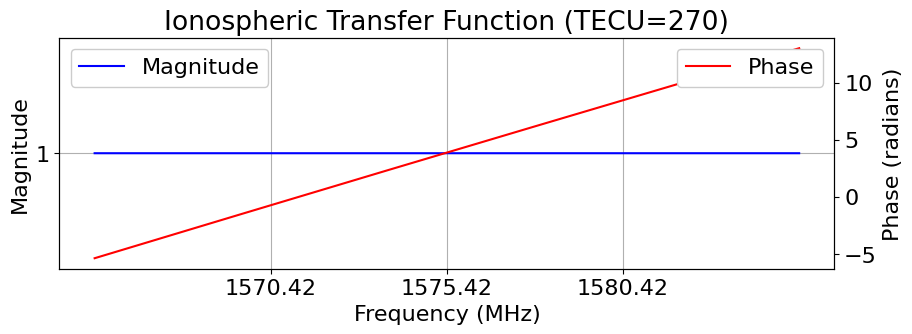
\includegraphics[width=0.8\linewidth]{img/iono-transfer-function.png}
    \caption{Example transfer function for ionospheric effect on L1 signal.}
    \label{fig:iono-freq-response}
\end{figure}

\begin{figure}
    \centering
    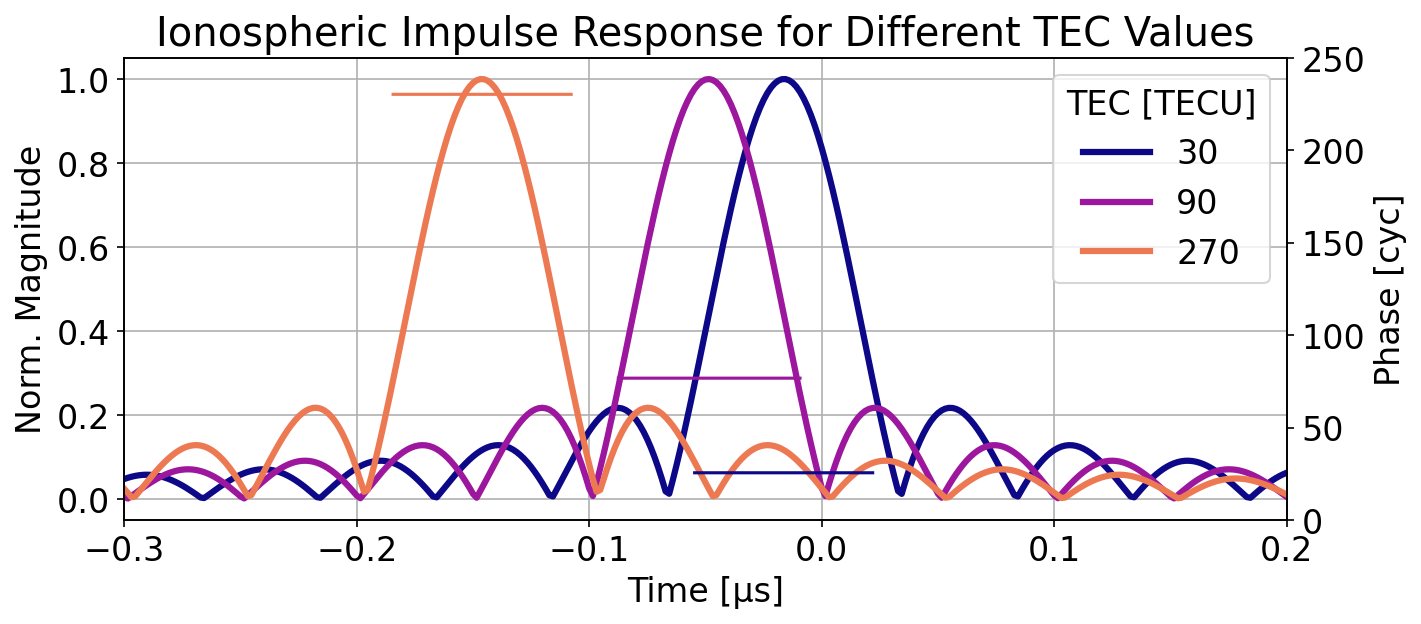
\includegraphics[width=0.8\linewidth]{img/iono-impulse-response.png}
    \caption{Example impulse responses for ionospheric effect on L1 signal for various TEC values.}
    \label{fig:iono-impulse-response}
\end{figure}

Working off of our sampled received baseband signal model from Equation \ref{eqn:received-sampled-signal-model}, we now refine our definition of propagation delay to include the dispersive group delays from both the ionosphere ($\tau_\text{iono}$) and transmitter/receiver hardware ($\tau_\text{hdwr}^\rho$):
%
\begin{align}
    \tau_\text{prop}(t) & = \tau_\text{range}(t) +
    \tau_\text{atmo}(t)+\tau_\text{iono}(t)+\tau^\rho_\text{hdwr}(t)
\end{align}
%
where $\tau_\text{range}$ is ``circularly defined'' as:
%
\begin{align}
    \tau_\text{range}(t) &=  \frac{1}{c} \cdot || \mathbf{r}_\text{tx}(t-\tau_\text{prop}(t))-\mathbf{r}_\text{rx}(t)||
\end{align}
%
Our apparent signal delay is now:
%
\begin{align}
    \tau_\rho(t) = \ &\Delta t_\text{rx}(t)-\Delta t_\text{tx}(t-\tau_\text{prop}(t)) \nonumber \\
    & + \tau_\text{range}(t) + \tau_\text{atmo}(t) + \tau_\text{iono}(t) + \tau_\text{hdwr}^\rho(t)
\end{align}
%
and our apparent phase delay is now:
%
\begin{align}
    \tau_\phi(t) = \ &\Delta t_\text{rx}(t)-\Delta t_\text{tx}(t-\tau_\text{prop}(t)) \nonumber \\
    & + \tau_\text{range}(t) + \tau_\text{atmo}(t) - \tau_\text{iono}(t) + \tau_\text{hdwr}^\phi(t)
\end{align}
%


\subsection{Non-Ideal Channel Models}







% More technically this:
% %
% \begin{align}
%     \frac{1}{c} \cdot P(t) = 
%     \tau_\eta(t) &= \Delta t_\text{rx}(t) - \Delta t_\text{tx}(t-\tau_\text{prop}(t)) + \tau_\text{nondisp}(t) + \tau_\text{iono}(t) + \tau_\text{hdwr,gr}(t)  \\
%     \frac{1}{c} \cdot \Phi(t) =
%     \tau_\phi(t) &= \Delta t_\text{rx}(t) - \Delta t_\text{tx}(t-\tau_\text{prop}(t)) + \tau_\text{nondisp}(t) - \tau_\text{iono}(t) + \tau_\text{hdwr,ph}(t)
% \end{align}
% %

% But approximately this is true:
% %
% \begin{align}
%     \Delta t_\text{tx}(t-\tau_\text{gr}(t)) \approx \Delta t_\text{tx}(t) - d_\text{tx}(t) \cdot \tau_\text{gr}(t)
% \end{align}
% %
% so therefore?
% %
% \begin{align}
%     \tau_\text{gr}(t) - d_\text{tx}(t) \cdot \tau_\text{gr}(t)
%     &= \Delta t_\text{rx}(t) - \Delta t_\text{tx}(t) + \tau_\text{nondisp}(t) + \tau_\text{iono}(t) + \tau_\text{hdwr,gr}(t)  \\
%     \Rightarrow \tau_\text{gr}(t) &= \frac{1}{1 - d_\text{tx}(t)} \left( \Delta t_\text{rx}(t) - \Delta t_\text{tx}(t) + \tau_\text{nondisp}(t) + \tau_\text{iono}(t) + \tau_\text{hdwr,gr}(t) \right)
% \end{align}
% %

% % approx
% %  C(eta_nondisp(0)+eta_dot*t) * exp(j*phi_nondisp(0)+j*omega*t)
% % -> C(eta_nondisp(0)+eta_disp+eta_dot*t) * exp(j*phi_nondisp(0)+j*phi_disp+j*omega*t)
% \begin{align}
%     \frac{1}{c} \cdot P(t) = 
%     \tau_\text{gr}(t) &= \Delta t_\text{rx}(t) - \Delta t_\text{tx}(t-\tau_\text{prop}(t)) + \tau_\text{iono}(t) + \tau_\text{hdwr,gr}(t)  \\
%     \frac{1}{c} \cdot \Phi(t) =
%     \tau_\text{ph}(t) &= \Delta t_\text{rx}(t) - \Delta t_\text{tx}(t-\tau_\text{gr}(t)) - \tau_\text{iono}(t) + \tau_\text{hdwr,ph}(t)
% \end{align}

% Received signal is now:
% %
% \begin{align}
%     s_\text{rx}[n] &= A_\text{rx}[n] \cdot C(t_\text{tx}(t[n]-\tau_\text{gr}[n])) \cdot \exp\left( j\cdot \left( t_\text{tx}(t[n]-\tau_\text{gr}[n])
% \end{align}

% In addition to group and phase delays, dispersive effects can cause signal distortion that lead to estimation errors when not accounted for properly.  Most prominently, 

% Correlation waveform distortion
% Can view as convolution of hardware channel response with ideal correlation response (due to linearity of convolution and correlation operations)
% There is technically a power and phase effect
% Often, signal distortion biases are absorbed into the hardware group delay and phase delay terms.  This is because, when close-loop tracked, the signal distortion bias remains constant and therefore indistinghishable from the net group delay and phase delay effects.  However, with open-loop tracking, without the DLL to drive code phase error towards zero, the distortion effect on magnitude and phase of correlation results can drift along with the OL model error.  (Illustrate with figure)


\section{Signal Structure}
% handle nav bits
% BPSK, TD-BPSK, BOC, MBOC, 


\section{Modeling}

\subsection{Oscillator}

\subsection{Orbit and Clock}

\subsection{Received Power, Antenna Gains, Losses, and Noise}

% TODO: handle more complex scenarios:
% 1. dispersion;  hardware dispersion leads to group delay and phase offset and code correlation response distortion;  ionosphere dispersion similarly produces a group delay, phase advance, and correlation response distortion (though we may simply model the group delay and carrier advance)
% 2. navigation data bits;  we assume our correlations occur over intervals where the navigation symbols or other unmodeled overlay symbols do not change
% 3. 


% TODO: handle modeling error assessment

% TODO: handle modeling itself:
%  Replica model is generated from model of signal delay (tau_d)
% This has contributions from:
% 1. propagation delay (range, atmospheric effects, non-clock hardware delays)
% 2. transmitter clock
% 3. receiver clock
% Transmitter/receiver positions and clock/oscillator offsets must be modeled and interpolated
% Sources of error (parameter estimate errors, timing errors, and linearization errors):
% 1. Clock prediction
% 2. Orbit/position prediction
% 3. Antenna offset/variations
% 4. Atmospheric/ionospheric effects

% One of the primary effects is receiver clock offset
% Ephemerides between different constellations need to be consistent;  need to handle constellation timing offset


\end{document}
